\chapter{Physics of Quarks and Gluons}

\section{The Standard Model}
\label{sec:sm}
The best widely adopted and tested description of the fundamental particles and their interactions is the \SM \cite{pdg}. 
\begin{figure}[htb]
    \centering
    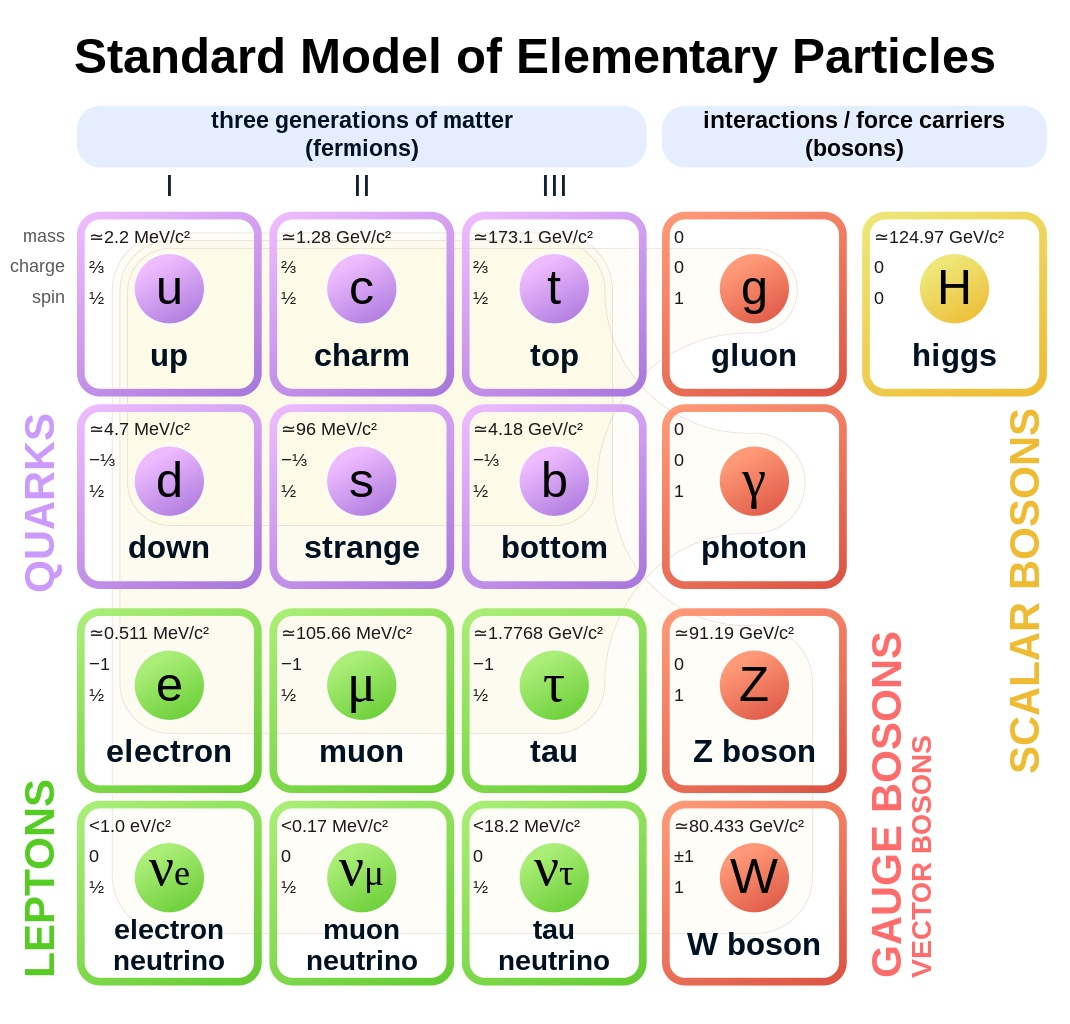
\includegraphics[width=0.6\linewidth]{src/img/sm.jpg}
    \caption[The Standard Model of particle physics.]{The Standard Model of particle physics. \footnotemark}
    \label{fig:sm}
\end{figure}
\footnotetext{\url{https://en.wikipedia.org/wiki/File:Standard_Model_of_Elementary(P)articles.svg}}
\emph{Fermions} are particles that makeup all the matter and \emph{bosons} are force-mediating particles.
All known elementary particles are displayed in \cref{fig:sm}.

Fermions are divided into two categories, \emph{leptons} and \emph{quarks}. 
Leptons are further divided into two groups:
\begin{enumerate}
    \item  
    \begin{itemize}
        \item \emph{electron}, a particle that is present in all matter around us,
        \item \emph{muon}, a heavier cousin of electron naturally produced in the atmosphere,
        \item \emph{tau lepton}, the heaviest lepton.
    \end{itemize}
    These three leptons can interact via the \emph{Electromagnetic Force} (they have a charge), mediated by \emph{photons}, or via the \emph{Weak force}, mediated by \emph{W and Z boson}. 
    \item \emph{Neutrinos}, each belonging to either electron, muon, or tau lepton.  
    Neutrinos can interact only weakly by exchanging W and Z bosons.
\end{enumerate}
Quarks are also divided into two groups:
\begin{multicols}{2}
\begin{enumerate}
    \item  
    With electric charge $\frac{2}{3}$ \footnote{Measured in units of elementary charge $e=1.60217663\cdot10^{-19}$ C.},
    \begin{itemize}
        \item \emph{up}, u quark,
        \item \emph{charm}, c quark,
        \item \emph{top}, t quark.
    \end{itemize}
    \item  
    With electric charge $-\frac{1}{3}$.
    \begin{itemize}
        \item \emph{down}, d quark,
        \item \emph{strange}, s quark,
        \item \emph{bottom}, b quark.
    \end{itemize}
\end{enumerate}
\end{multicols}
All quarks can interact weakly and electromagnetically via the \emph{Strong Force}, mediated by \emph{gluons}.
In nature, practically only the u-quark and d-quark occur. 
Concretely, they are the building blocks of protons and neutrons.

Fermions can be also split another way, into three families (\emph{generations}). 
The mass of corresponding particles gives the order of families.
The lightest is built up by a u-quark, a d-quark, an electron, and an electron neutrino.
Practically all matter around us is made up of particles from this family.
It should be noted that neutrino masses are not precisely known.
Due to a measured process \cite{sadbury} called neutrino oscillations \cite{pdg}, they cannot be massless.
Since the first discovery, estimates on the upper bound of their masses were made \cite{pdg}.

The bosonic particles are a photon, gluon, W, and Z boson, and \emph{Higgs boson}. They can be split up into two groups:
\begin{enumerate}
    \item \emph{Vector Bosons}: photon, gluon, W and Z boson,
    \item \emph{Gauge Bosons}: Higgs boson.
\end{enumerate}
Vector bosons ('vector' comes from their mathematical description) are force carriers:
\begin{itemize}
    \item \emph{Electromagnetic Force} - photon,
    \item \emph{Strong Force} - gluon,
    \item \emph{Weak Force} - Z and W boson.
\end{itemize}
The properties of the corresponding force-carrying boson give the nature of each force.
The corresponding charge of interacting particles gives the interaction strength of each force.

Particles that have electric charges can exchange photons and interact electromagnetically.
The infinite range of the Electromagnetic force is due to the massless photons.
They also have no charge, which makes them unable to scatter on other photons.~\footnote{This has some caveats at higher energies. Classically it is forbidden due to the linearity of Maxwell's equations, but at higher orders of perturbation QFT, photons can scatter on another photon. However, the probability of such an event is very low.}

Gluons are also massless, making the Strong force also infinite.
Quarks are the only fermion carriers of the strong charge (also called \emph{color charge}). 
Since gluons have two strong chargers, they can interact with other gluons and exchange color charges when interacting with quarks or gluons.
This differs from Electromagnetic Interaction, where particles' charge does not change. 
Even though the Strong interaction is theoretically infinite, we do not see free gluons or quarks due to a process called \emph{hadronization} (detailed description in ????). 
They only occur in a bound state in nature, effectively making the color charge invisible at a larger scale (it becomes visible at~the~scale~of approximately 1 fm)

All fermions can interact weakly, but since W and Z bosons have mass (which is significant compared to fermions), the range of interaction is short.
Weak processes occur, for example, in $\beta$-decay.

Last but not least is the Higgs boson, a scalar boson.
The strength of the interaction with the Higgs boson (more precisely: with the scalar field, Higgs field) is given by the mass of the interacting particle.
In other words, particles' interaction with the Higgs field gives them mass.
Gluons and photons are the only particles from \SM non-interacting with the Higgs boson.



\section{Quantum Field Theory}
\label{sec:qft}
\QFT is a fundamental framework in modern theoretical physics that describes the behavior of particles and fields at the quantum level.
Paul Dirac did the first development by studying the electromagnetic interaction of particles and photons by \cite{dirac}.
Massive progress in \QED did Richard Feynman \cite{feynman}, who also introduced the \emph{Feynman diagrams}, a graphical representation of interactions.
We will discuss Feynman diagrams in more detail in \cref{sec:feyman}.

The starting point of QFT is that particles are not fundamental objects but excitations of underlying quantum fields that permeate all of space and time. 
This field must satisfy the equations of motion of the corresponding field theory derived from the Lagrangian density of the theory.

\subsection{Free Particles}
\label{sec:free_particles}
The Lagrangian of non-interacting \spinhalf particle, also called the \emph{Dirac Lagrangian}, is given by
\begin{equation}
    \label{eq:dirac_lag}
    \mathcal{L}_{\text{Dirac}} = \bar{\psi}(i\slashed{\partial} - m) \psi,
\end{equation}
where we abbreviate $\gamma^\mu \partial_\mu \equiv \slashed{\partial}$, $\gamma^\mu$ are the Dirac matrices, and $\partial_\mu$ is the covariant derivative.
$\psi(x)$ is a bispinor fermionic field of a spin $\frac{1}{2}$ particle. 
It has four components, which can be split into two spinors, each corresponding to a different chirality
\begin{equation}
    \psi(x) = \left( \begin{array}{c} \psi_L(x) \\ \psi_R(x) \end{array} \right).
\end{equation}
Going further we will always abbreviate $\gamma^\mu V_\mu \equiv \slashed{V}$, where $V$ is a 1-form or a vector with lowered indices $V_\mu = \eta_{\mu \nu} V^\nu$ with the Minkowski metric $\eta_{\mu \nu} = \text{diag}(1,-1,-1,-1)$. 
We also automatically sum over repeated indices, utilizing the Einstein summation convention.
The Dirac equation is an equation of motion derived from the Lagrangian \cref{eq:dirac_lag}:
\begin{equation}
    \label{eq:dirac}
    \left( i \gamma^\mu \partial_\mu - m \right) \psi(x) = 0.
\end{equation}
It can be solved analytically.

The solutions to this equation describe how fermion particles propagate in space and time without interaction. 

Conversely, bosons are spin-1 particles, described by the vector field $A_\mu(x)$.
The Lagrangian of a non-interacting spin-1 particle is given by a \emph{Proca Lagrangian}
\begin{equation}
    \label{eq:proca_lag}
    \mathcal{L}_{\text{Proca}} = - \frac{1}{4} F_{\mu\nu} F^{\mu\nu} + \frac{1}{2} m^2 A_\mu A^\mu,
\end{equation}
where $F_{\mu\nu} = \partial_\mu A_\nu - \partial_\nu A_\mu$ is the field strength tensor.
Note that this Lagrangian describes massive bosons. 
In the case of massless bosons, the second term is omitted.
The equation of motion for the vector field, the Klein-Gordon equation, follows from the Lagrangian \cref{eq:proca_lag}
\begin{equation}
    \label{eq:klein_gordon}
    \left( \Box + m^2 \right) A_\mu(x) = 0.
\end{equation}
The solutions to this equation can also be found analytically.
In the case of massless bosons, the equation reduces to 
\begin{equation}
    \label{eq:wave_eq}
    \Box A_\mu(x) = 0,
\end{equation}
which is a simple wave equation.
We can rewrite it using the field strength tensor as
\begin{equation}
    \Box A_\mu(x) = \partial_\nu \partial^\nu A_\mu(x) = \partial_\nu \partial_\nu A_\mu(x) - \partial_\nu \partial_\mu A_\mu(x) =  \partial_\nu F_{\nu\mu}(x) =  0,
\end{equation}
which are Maxwell's equations, meaning that massless non-interacting bosons propagate the same way as electromagnetic waves.
We have utilized the Lorentz gauge $\partial_\mu A_\mu(x) = 0$.


\subsection{Interacting Particles}
\label{sec:interacting_particles}
We introduce the interaction between fields by invoking the \emph{local gauge invariance} of the Lagrangian. 

Each type of interaction (strong, electromagnetic, weak) corresponds to a different $SU(N)$ \emph{Lie group} \cite{fecko}.
Elements of $SU(N)$ are special unitary $N$x$N$ matrices \footnote{Matrix U is special if det$U=1$ and unitary if $UU^{\dagger} = 1$}. 
When operating on $N$-dimensional space of fields, they are represented as unitary operators in the form 
\begin{equation}
    \label{eq:lie_element}
    U = \eu^{i g \sum_{a} \alpha^a T^a},
\end{equation}
where $T^a$ are generators of the group, and $\alpha^a$ and $g$  are the parameters of the transformation.
For example, in the case of a rotating spinor in classical quantum mechanics, the group is the rotation group SU(2), and the generators are the Pauli matrices $T^a \equiv \frac12 \hat{\sigma}_a$ ($a = x,y,z$).
$g$ would be the angle of rotation, and $\alpha^a \equiv \vec{n}$ is the axis of rotation.
More generally, $T^a$ can be represented as $N$x$N$ matrices, where $N$ is the field space dimension.
Going further, we will suppress writing the summation over $a$ (or any other index) explicitly unless it is necessary for clarity.
The generators satisfy the commutation relations
\begin{equation}
    \label{eq:commutation}
    [T^a, T^b] = i f^{abc} T^c,
\end{equation}
where $f^{abc}$ are the structure constants of the Lie group.

A Lagrangian describes an interacting physical system if it is invariant under the local gauge transformation
\begin{equation}
    \label{eq:}
    \psi_j(x)' = U_{ij}(x)\psi(x)_j = \eu^{i g \alpha^a(x) T^a_{ij}} \psi(x)_j,
\end{equation}
of the spinor quantum fields $\psi(x)_i$, and under the infinitesimal transformation of the vector fields $A^a_\mu(x)$
\begin{equation}
    \label{eq:gauge_inv_bosons}
    A^a_\mu(x)' \rightarrow A^a_\mu(x) + \frac{1}{g} \partial_\mu \alpha^a(x) - f^{abc} \alpha^b(x) A^c_\mu(x) + \mathcal{O}((f^{abc})^2),
\end{equation}
where $U(x)$ is an element of the corresponding Lie group for every spacetime point $x$.
$g$ is the coupling constant of the interaction, and $\alpha^a(x)$ are the parameters of the transformation.


For example, the electromagnetic interaction corresponds to the $U(1)$ group (Lie group isomorphic to complex numbers), which means that the Lagrangian must be invariant under the transformations
\begin{equation}
    \label{eq:gauge_inv_QED}
    \psi(x) = \eu^{-i e \alpha(x)}\psi(x) \quad, \quad A_\mu(x) = A_\mu(x) + \frac{1}{e} \partial_\mu \alpha(x).
\end{equation}
where the a generator of the $U(1)$ group is just a constant $T^a = 1$, so the structure constants are zero $f^{abc} = 0$.

In the general case of the non-Abelian $SU(N)$ group having $N$ different fermions with the free Lagrangian
\begin{equation}
    \label{eq:Dirac_N}
    \mathcal{L}_{\text{Dirac}} = \sum_{i=1}^N \bar{\psi}_i (i\slashed{\partial} - m) \psi_i,
\end{equation}
the local gauge invariant Lagrangian is given by \cite{schartz}
\begin{equation}
    \label{eq:lag_suN}
    \mathcal{L} = - \frac{1}{4}  G^a_{\mu\nu} G^a_{\mu\nu} + \frac{1}{2} m^2 A^a_\mu A^a_\mu, + \sum_{i,j=1}^N \bar{\psi}_i (i\delta_{ij} \slashed{\partial}  +g \slashed{A}^a T^a_{ij} - m \delta_{ij}) \psi_j.
\end{equation}
where the field strength tensor is modified, as a result of the non-commutativity of the generators, to
\begin{equation}
    \label{eq:field_strength}
    G^a_{\mu\nu} = F^a_{\mu\nu} + g f^{abc} A^b_\mu A^c_\nu = \partial_\mu A^a_\nu - \partial_\nu A^a_\mu + g f^{abc} A^b_\mu A^c_\nu,
\end{equation}
such that it preserves the local gauge invariance.
This additional term significantly impacts the system's dynamics because the last term corresponds to boson-boson interaction.
We shall see in \cref{sec:QCD} the consequences of this interaction.

To go back to the example of the $U(1)$, the corresponding Lagrangian has the form \footnote{$G^a_{\mu\nu} \equiv F^a_{\mu\nu}$, because $f^{abc} = 0$}
\begin{equation}
    \label{eq:qed_lag}
    \mathcal{L} = - \frac{1}{4}  F_{\mu\nu} F_{\mu\nu} + \bar{\psi}(i\slashed{\partial} - m) \psi - e \bar{\psi} \gamma^\mu \partial_\mu \psi A_\mu.
\end{equation}
The equations of motion of the Lagrangian (\ref{eq:qed_lag}) ultimately determine the system's dynamics.

\subsection{Cross Section}
\label{sec:cross_section}
In particle physics, we are not interested in calculating the actual state $psi(x)$ as a solution to the equations of motion of the Lagrangian (\ref{eq:qed_lag}), but rather in the probability of two particles interacting. 
The physical quantity describing this probability is the cross section $\sigma$.
With the probabilistic nature of quantum mechanics, we need to define this quantity based on more interactions.
Suppose we have a flux of incoming particles scattered off target particles. 
Then the probability that a given particle will scatter off of a target particle is given as 
\begin{equation}
    \label{eq:cross_sec}
    \sigma = \frac{\text{number of scattered particles}}{\text{incoming flux of particles}},
\end{equation}
where the flux has units m$^{-2}$ so the cross section has units m$^{2}$.

If we want to specify the infinitesimal probability of particles scattering to a space angle d$\Omega$, we can define it as
\begin{equation}
    \label{eq:diff_cross_sec}
    d\sigma = \frac{\text{number of scattered particles to an space angle } d\Omega}{\text{incoming flux of particles}}.
\end{equation}
Or, if we want the cross section in terms of the momentum of the scattered particles d$p$, we can define it as 
\begin{equation}
    \label{eq:diff_cross_sec_p}
    d\sigma = \frac{\text{number of scattered particles with outgoing momentum } dp}{\text{incoming flux of particles}}.
\end{equation}

Quantum mechanically, we expect the cross section to be given by the probability of the system being in a final state $|f\rangle$ given that it was in the initial state $|i\rangle$.
We can express this as 
\begin{equation}
    \label{eq:cross_sec_qm}
    \sigma \sim |\langle f | \eu^{-i \hat{H} (t_{out} - t_{in})} | i \rangle |^2,
\end{equation}
where $\hat{H}$ is the Hamiltonian of the system, and $t_{in}$ and $t_{out}$ are the initial and final times of the system.

To be more precise, for two interacting particles with energies $E_{1,{\text{in}}}$, $E_{2,{\text{in}}}$ and velocities $\vec{v}_{1,{\text{in}}}$, $\vec{v}_{2,{\text{in}}}$, and $N$ particles in the final state with energies $E_{j,{\text{out}}}$ ($j=1,2,..., N$), we can write \cite{schartz}
\begin{equation}
    \label{eq:cross_sec_qft}
    d \sigma = \frac{|\mathcal{M}|^2}{4 E_{1,{\text{in}}} E_{2,{\text{in}}} |\vec{v}_{1,{\text{in}}} - \vec{v}_{2,{\text{in}}}|} (2\pi)^4 \delta^4(p^\mu_{\text{in}} - p^\mu_{\text{out}}) \prod_{j=1}^N \frac{d^3 p_j}{(2\pi)^3 2E_{j, {\text{out}}}}, 
\end{equation}
where $p^\mu_{\text{in}}$ is the 4-momentum of the incoming particles and $p^\mu_{\text{out}}$ is the 4-momentum of the outgoing particles, the $\delta^4(p^\mu_{\text{in}} - p^\mu_{\text{out}})$ function is the 4-dimensional Dirac delta function enforcing 4-momentum conservation, and the $|\mathcal{M}|^2$ is the matrix element of the \emph{scattering amplitude} $\mathcal{M}$.
The matrix element $\langle f |\mathcal{M} | i \rangle$ (where $|\mathcal{M}|^2 \equiv |\langle f |\mathcal{M} | i \rangle |^2$) is given by (assuming $ | f \rangle \neq | i \rangle$)
\begin{equation}
    \label{eq:M_matrix}
    \langle f | S | i \rangle = i (2\pi)^4 \delta^4(p^\mu_{\text{in}} - p^\mu_{\text{out}})  \langle f | \mathcal{M} | i \rangle,
\end{equation}
where $S$ is the $S$-matrix of the scattering process.
We can calculate the $S$-matrix utilizing the Dyson series expansion \cite{schartz}
\begin{equation}
    \label{eq:s_dyson}
    \langle f | S | i \rangle =\left\langle f \left|\sum_{n=0}^{\infty} \frac{(-i)^n}{n !} \int d x_1^4 \cdots \int d x_n^4 T\left[\mathcal{H}\left(t_1\right) \cdots \mathcal{H}\left(t_n\right)\right]\right| i \right\rangle,
\end{equation}
where $T\left[\mathcal{H}\left(t_1\right) \cdots \mathcal{H}\left(t_n\right)\right]$ is the time-ordered product of the Hamiltonian of the system, and $\mathcal{H}$ is the Hamiltonian density of the system.
Equation (\ref{eq:cross_sec_qm}) is a particular case of equation (\ref{eq:s_dyson}) where the Hamiltonian is time-independent.


\subsection{Feynman Diagrams}
\label{sec:feyman}
Calculating the expansion (\ref{eq:s_dyson}) is practically impossible analytically, so Feynman developed a graphical method to calculate individual terms.
The diagrams consist of the following:
\begin{itemize}
    \item \textbf{External lines} represent the incoming and outgoing particles, which are \emph{real} particles,
    \item \textbf{Internal lines} represent the intermediate particles, which are \emph{virtual} particles,
    \item \textbf{Vertices} are the points of interaction.    
\end{itemize}
Virtual particles are not real particles but mathematical construct that allows us to visualize the scattering process.
Each part contributes a multiplicative factor to the amplitude $-i\mathcal{M}$.
The \emph{order of the diagram} is the number of interaction vertices and the order of the term in the Dyson series expansion.

\begin{figure}[htb]
\begin{tikzpicture}
    \begin{feynman}
        \vertex (a);
        \vertex [below =of a](c);
        \vertex [above left=of a] (i1) {\(\mu^{-}, p_1\)};
        \vertex [above right=of a] (f1) {\(\mu^{-}, p_3\)};
        \vertex [below left=of c] (i2) {\(e^{-}, p_2\)};
        \vertex [below right=of c] (f2) {\(e^{-}, p_4\)};
        \diagram* {
            (i1) -- [fermion] (a) -- [fermion] (f1),
            (a) -- [photon, edge label=\(\gamma\), momentum'=\(p_\gamma\)] (c),
            (i2) -- [fermion] (c) -- [fermion] (f2),
        };
    \end{feynman}
\end{tikzpicture}
\caption{Second-order Feynman diagram of electron-muon scattering.}
\label{fig:electron_muon}
\end{figure}
To give an example, we consider electron-muon scattering.
The second-order Feynman diagram for this process, shown in \cref{fig:electron_muon}, is the lowest-order diagram that can contribute to the cross section.

The time flows from left to right, so we have an incoming electron and muon. 
They exchange a virtual photon, momentum, and scatter.
The incoming particles, with momenta $p_1$, $p_2$, contribute factors $u(p_1)$, $u(p_2)$, which are solutions to the free Dirac equation (\ref{eq:dirac}) in momentum space. 
The outgoing particles, with momenta $p_3$, $p_4$, contribute factors $\bar{u}(p_3)$, $\bar{u}(p_4)$, which are complex conjugates of the free Dirac equation solutions.
The vertex is where interaction happens, and corresponding term $ie\gamma^\mu$ is given by the interaction Lagrangian $\mathcal{L}_{\text{int}} = - e \bar{\psi} \gamma^\mu \partial_\mu \psi A_\mu$.
Virtual photon, with momentum $p_{\gamma}$, is an internal line, its contribution is $\frac{-i\eta_{\mu \nu}}{p_{\gamma}^2}$.
We can now write the amplitude as 
\begin{equation}
    \label{eq:e_mu_amp}
    -i\mathcal{M} = \bar{u}(p_3) (ie\gamma^\mu) u(p_1) \frac{-i\eta_{\mu \nu}}{p_{\gamma}^2} \bar{u}(p_4) (ie\gamma^\nu) u(p_2)
\end{equation}
Utilizing the conservation of momentum, we can write $p_{\gamma} = p_1 - p_3$, we can write
\begin{equation}
    \label{eq:e_mu_amp_2}
    \mathcal{M} = -e^2 \bar{u}(p_3) \gamma^\mu u(p_1) \frac{1}{(p_1 - p_3)^2} \bar{u}(p_4) \gamma_\mu u(p_2).
\end{equation}
After multiplying by the complex conjugate, summing over all the possible spins, and neglecting masses of electron and muon (we assume relativistic scattering), we can write the matrix element as
\begin{equation}
    |\mathcal{M}|^2 = 2e^4\frac{(p_1 + p_2)^2 + (p_1 - p_4)^2}{(p_1 - p_3)^2}.
\end{equation}
We can now evaluate the cross section (\ref{eq:cross_sec_qft}) in the centre of mass frame as
\begin{equation}
    \label{eq:cross_sec_qft_2}
    \frac{d\sigma}{d\Omega} = \frac{\alpha^2}{4(p_1 + p_2)^2} (1+\cos^2{\theta}),
\end{equation}
where $\theta$ is the scattering angle.
Integrating over the solid angle, we get the total cross section
\begin{equation}
    \sigma =  \frac{4\pi\alpha^2}{3(p_1 + p_2)^2}.
\end{equation}

\begin{figure}[htb]
    \begin{subfigure}[t]{0.4\textwidth}
        \begin{tikzpicture}
            \begin{feynman}
                \vertex (a);
                \vertex [below =of a](c);
                \vertex [right =of a](b);
                \vertex [right =of c](d);
                \vertex [above left=of a] (i1) {\(\mu^{-}\)};
                \vertex [above right=of b] (f1) {\(\mu^{-}\)};
                \vertex [below left=of c] (i2) {\(e^{-}\)};
                \vertex [below right=of d] (f2) {\(e^{-}\)};
                \diagram* {
                    (i1) -- [fermion] (a) -- [fermion] (b) -- [fermion] (f1),
                    (a) -- [photon] (c),
                    (b) -- [photon] (d),
                    (i2) -- [fermion] (c) -- [fermion] (d) -- [fermion] (f2),
                };
            \end{feynman}
        \end{tikzpicture}
        \caption{}
        \label{fig:e_mu_higher_a}
    \end{subfigure}
    \begin{subfigure}[t]{0.4\textwidth}
        \begin{tikzpicture}
            \begin{feynman}
                \vertex (a);
                \vertex [below =of a](c);
                \vertex [right =of a](b);
                \vertex [right =of c](d);
                \vertex [above left=of a] (i1) {\(\mu^{-}\)};
                \vertex [above right=of b] (f1) {\(\mu^{-}\)};
                \vertex [below left=of c] (i2) {\(e^{-}\)};
                \vertex [below right=of d] (f2) {\(e^{-}\)};
                \diagram* {
                    (i1) -- [fermion] (a) -- [fermion] (b) -- [fermion] (f1),
                    (a) -- [photon] (d),
                    (b) -- [photon] (c),
                    (i2) -- [fermion] (c) -- [fermion] (d) -- [fermion] (f2),
                };
            \end{feynman}
        \end{tikzpicture}
        \caption{}
        \label{fig:e_mu_higher_b}
    \end{subfigure}
    \caption{Fourth order Feynman diagram for electron-muon scattering.}
    \label{fig:e_mu_higher}
\end{figure}


This calculation was an example of the lowest-order Feynman diagram.
In general, many more diagrams contribute to the amplitude, \cref{fig:electron_muon} is a fourth-order diagram.

The \emph{Feynman rules} for the general \QED Feynman diagram can be found in \cite{intro_to_part}.
Other interactions have slightly different Feynman rules, but the general idea is the same.


\section{Quantum Chromodynamics}
\label{sec:QCD}
So far, we have introduced \QED interactions as examples. 
In this section, we will introduce \QCD, the theory of strong interactions.
The underlying Lie group of \QCD is  $SU(3)$.
We can derive the following from the general theory introduced in \cref{sec:interacting_particles}. 
$N=3$, which means the underlying field space is three-dimensional.
Physically, we have \textbf{3 quark fields} for each quark in the \SM.
They correspond to 3 color states $\psi_i(x)$, $i=1,2,3$.
$SU(3)$ has 8 generators $T^a$, which means we have \textbf{8 gluon fields} $A^a_\mu(x)$, $a=1,\dots, 8$.
The full Lagrangian of \QCD is \cite{qcd} (we also suppress the summation over quark fields $i,j$)
\begin{align}
\begin{split}
    \label{eq:qcd_lag}
    \mathcal{L}_{\text{QCD}}  &= - \frac{1}{4}  G^a_{\mu\nu} G^a_{\mu\nu}  + \bar{\psi}_i (i \slashed{\partial} - m ) \psi_i + g \bar{\psi}_i \slashed{A}^a T^a_{ij} \psi_j \\
     &= - \frac{1}{4}  F^a_{\mu\nu} F^a_{\mu\nu}  + \bar{\psi}_i (i \slashed{\partial} - m ) \psi_i + g \bar{\psi}_i \slashed{A}^a T^a_{ij} \psi_j + \\    
     &+ g f^{a b c}\left[\left(\partial_\mu A_\nu^a-\partial_\nu A_\mu^a\right) A_b^\mu A_c^\nu+\left(\partial_\mu A^{a\nu}-\partial_\nu A^{a \mu}\right) A_{b \mu} A_{c \nu}\right] + \\
     &+ g^2 f^{a b c} f^{a d e} A_b^\mu A_c^\nu A_{d \mu} A_{e \nu},
\end{split}
\end{align}
where we have expanded $G^a_{\mu\nu}$ as in (\ref{eq:field_strength}). 
We can now see that the two last terms correspond to three and four-gluon coupling.


\subsection{Feynamn Diagrams of QCD}
The complete list of Feynman rules for \QCD can be found in \cite{qcd}.
However, we will introduce some of the essential Feynman diagrams here.

\subsubsection*{Quark-quark scattering}
Lowest order diagrams for quark-quark scattering are shown in \cref{fig:qq}.
Quarks have the same type of 'fermionic' line as leptons discussed in \cref{sec:qft}.
Gluons are represented with 'curly' lines to distinguish the strong interaction from the electromagnetic.
The possibility of the initial quarks having different color charges adds magnitude to the overall amplitude because we need to sum over all possibilities. 
To illustrate this, we take a look at a fraction of cross section of $e^+ e^- \rightarrow$ hadrons and $e^+ e^- \rightarrow \mu^+ \mu^-$
\begin{equation}
    R = \frac{\sigma(e^+ e^- \rightarrow \text{hadrons})}{\sigma(e^+ e^- \rightarrow \mu^+ \mu^-)},
\end{equation}
if we do not sum over the color charges, the fraction is $2/3$, but if we do sum over the color charges, the fraction is $2$
\begin{equation}
    R_{\text{no color}} = \frac{2}{3}, \quad R_{\text{color}} = 2.
\end{equation}


\begin{figure}[htb]
    \centering
    \begin{subfigure}[t]{0.49\textwidth}
        \centering
        \begin{tikzpicture}
            \begin{feynman}
                \vertex (a);
                \vertex [below =of a](c);
                \vertex [above left=of a] (i1) {\(q_1\)};
                \vertex [above right=of a] (f1) {\(q_1\)};
                \vertex [below left=of c] (i2) {\(q_2\)};
                \vertex [below right=of c] (f2) {\(q_2\)};
                \diagram* {
                    (i1) -- [fermion] (a)  -- [fermion] (f1),
                    (a) -- [gluon] (c),
                    (i2) -- [fermion] (c)  -- [fermion] (f2),
                };
            \end{feynman}
        \end{tikzpicture}
        \caption{}
        \label{fig:qq_a}
    \end{subfigure}
    \begin{subfigure}[t]{0.49\textwidth}
        \centering
        \begin{tikzpicture}
            \begin{feynman}
                \vertex (a);
                \vertex [below =of a](c);
                \vertex [above left=of a] (i1) {\(q_1\)};
                \vertex [above right=of a] (f1) {\(q_2\)};
                \vertex [below left=of c] (i2) {\(q_2\)};
                \vertex [below right=of c] (f2) {\(q_1\)};
                \diagram* {
                    (i1) -- [fermion] (a)  -- [fermion] (f2),
                    (a) -- [gluon] (c),
                    (i2) -- [fermion] (c)  -- [fermion] (f1),
                };
            \end{feynman}
        \end{tikzpicture}
        \caption{}
        \label{fig:qq_b}
    \end{subfigure}
    \caption{Lowest-order Feynman diagrams of quark-quark scattering.}
    \label{fig:qq}
\end{figure}


\subsubsection*{Quark-gluon scattering}
The lowest order diagrams for quark-gluon scattering are shown in \cref{fig:qg}.
Due to the gluon self-interaction, there are more diagrams than in \QED.
\begin{figure}[htb]
    \centering
    \begin{subfigure}{0.4\textwidth}
        \centering
        \begin{tikzpicture}
            \begin{feynman}
                \vertex (a);
                \vertex [right =of a](c);
                \vertex [below left=of a] (i1) {\(g\)};
                \vertex [above left=of a] (i2) {\(q\)};
                \vertex [below right=of c] (f2) {\(g\)};
                \vertex [above right=of c] (f1) {\(q\)};
                \diagram* {
                    (i1) -- [gluon] (a),
                    (i2) -- [fermion] (a),
                    (a) -- [fermion] (c),
                    (c)   -- [fermion](f1), 
                    (c) -- [gluon] (f2),
                };
            \end{feynman}
        \end{tikzpicture}
        \caption{}
        \label{fig:qg_a}
    \end{subfigure}
    \begin{subfigure}[t]{0.29\textwidth}
        \centering
        \begin{tikzpicture}
            \begin{feynman}
                \vertex (a);
                \vertex [below =of a](c);
                \vertex [above left=of a] (i1) {\(q\)};
                \vertex [above right=of a] (f1) {\(g\)};
                \vertex [below left=of c] (i2) {\(g\)};
                \vertex [below right=of c] (f2) {\(q\)};
                \diagram* {
                    (i1) -- [fermion] (a)  -- [gluon] (f1),
                    (a) -- [fermion] (c),
                    (i2) -- [gluon] (c)  -- [fermion] (f2),
                };
            \end{feynman}
        \end{tikzpicture}
        \caption{}
        \label{fig:qg_b}
    \end{subfigure}
    \begin{subfigure}[t]{0.29\textwidth}
        \centering
        \begin{tikzpicture}
            \begin{feynman}
                \vertex (a);
                \vertex [below =of a](c);
                \vertex [above left=of a] (i1) {\(q\)};
                \vertex [above right=of a] (f1) {\(q\)};
                \vertex [below left=of c] (i2) {\(g\)};
                \vertex [below right=of c] (f2) {\(q\)};
                \diagram* {
                    (i1) -- [fermion] (a)  -- [fermion] (f1),
                    (a) -- [gluon] (c),
                    (i2) -- [gluon] (c)  -- [gluon] (f2),
                };
            \end{feynman}
        \end{tikzpicture}
        \caption{}
        \label{fig:qg_c}
    \end{subfigure}
    \caption{Lowest-order Feynman diagrams of quark-gluon scattering.}
    \label{fig:qg}
\end{figure}

\subsubsection*{Gluon-gluon scattering}
The lowest order diagrams for gluon-gluon scattering are shown in \cref{fig:gg}.
In \QCD, gluons can interact directly with each other.
These interactions are non-trivial. 
A theory called \emph{gluodynamics} is developed to describe just gluon-gluon interactions.
In \cref{fig:gg_a} and \cref{fig:gg_b}, we can see the 3-gluon vertex, and in \cref{fig:gg_c}, we can see the 4-gluon vertex.

\begin{figure}[htb]
    \centering
    \begin{subfigure}{0.4\textwidth}
        \centering
        \begin{tikzpicture}
            \begin{feynman}
                \vertex (a);
                \vertex [right =of a](c);
                \vertex [below left=of a] (i1) {\(g\)};
                \vertex [above left=of a] (i2) {\(g\)};
                \vertex [below right=of c] (f2) {\(g\)};
                \vertex [above right=of c] (f1) {\(g\)};
                \diagram* {
                    (i1) -- [gluon] (a),
                    (i2) -- [gluon] (a),
                    (a) -- [gluon] (c),
                    (c)   -- [gluon](f1), 
                    (c) -- [gluon] (f2),
                };
            \end{feynman}
        \end{tikzpicture}
        \caption{}
        \label{fig:gg_a}
    \end{subfigure}
    \begin{subfigure}[t]{0.29\textwidth}
        \centering
        \begin{tikzpicture}
            \begin{feynman}
                \vertex (a);
                \vertex [below =of a](c);
                \vertex [above left=of a] (i1) {\(g\)};
                \vertex [above right=of a] (f1) {\(g\)};
                \vertex [below left=of c] (i2) {\(g\)};
                \vertex [below right=of c] (f2) {\(g\)};
                \diagram* {
                    (i1) -- [gluon] (a)  -- [gluon] (f1),
                    (a) -- [gluon] (c),
                    (i2) -- [gluon] (c)  -- [gluon] (f2),
                };
            \end{feynman}
        \end{tikzpicture}
        \caption{}
        \label{fig:gg_b}
    \end{subfigure}
    \begin{subfigure}[t]{0.29\textwidth}
        \centering
        \begin{tikzpicture}
            \begin{feynman}
                \vertex (a);
                \vertex [above left=of a] (i1) {\(g\)};
                \vertex [above right=of a] (f1) {\(g\)};
                \vertex [below left=of a] (i2) {\(g\)};
                \vertex [below right=of a] (f2) {\(g\)};
                \diagram* {
                    (i1) -- [gluon] (a)  -- [gluon] (f1),
                    (i2) -- [gluon] (a)  -- [gluon] (f2),
                };
            \end{feynman}
        \end{tikzpicture}
        \caption{}
        \label{fig:gg_c}
    \end{subfigure}
    \caption{Lowest-order Feynman diagrams of gluon-gluon scattering.}
    \label{fig:gg}
\end{figure}

\subsubsection*{Gluon Emission}
Let's consider a $e^+e^-$ annihilation process producing two quarks, and one of the quarks emits a real gluon.
\begin{figure}[htb]
        \centering
        \begin{tikzpicture}
            \begin{feynman}
                \vertex (a);
                \vertex [right =of a](c);
                \vertex [above right =of c](d);
                \vertex [above right=of d] (f2) {\(q_1\)};
                \vertex [right=of d] (f3) {\(g\)};
                \vertex [below right=of c] (f1) {\(q_2\)};
                \diagram* {
                    (a) -- [photon] (c),
                    (c) -- [fermion](d),
                    (d) -- [fermion](f2),
                    (d) -- [gluon](f3), 
                    (c) -- [fermion] (f1),
                };
            \end{feynman}
        \end{tikzpicture}
    \caption{Lowest-order Feynman diagram of quark emitting a gluon.}
    \label{fig:qg_emission}
\end{figure}
We will only look at the right part of the diagram after the annihilation, as seen in \cref{fig:qg_emission}.
The scattering amplitude is given by \cite{qcd}
\begin{equation}
    \label{eq:g_emission}
    \mathcal{M}_{q \bar{q} g}^\mu=\bar{u}\left(p_1\right)\left(-i g T^a \slashed{\epsilon} \right) \frac{i\left(\slashed{p_1} +\slashed{k}\right)}{\left(p_1+k\right)^2}\left(-i e \gamma^\mu\right) v\left(p_2\right) ,
\end{equation}
where $p_1$, $p_2$ are the momenta of the quarks $q_1$, $q_2$, $k$ is the momentum of the gluon, and $\epsilon$ is the solution of a free gluon.



\section{Infrared and Collinear Divergences}
\label{sec:IR_div}
The perturbation expansion (\ref{eq:s_dyson}) is done in the constant of interaction $g$. 
However, the assumption of $g$ being a constant is not valid.
It changes with the energy of the particles, hence the distance between them. 
In \QED, we have the \emph{asymptotic freedom}, which means the coupling constant $g$ goes to zero as the distance between the particles goes to infinity.
The coupling constant grows when we force particles to be closer to each other by smashing them together with high enough energy.
In \QCD, the coupling constant grows with the distance between the quarks.
The difference arises because, in \QCD, there are three quark color fields, whereas, in \QED, there is only one.
The structure given by the Lie group $SU(3)$ dramatically changes the behavior of the coupling constant.
Another way to formulate this is that the probability of a quark emitting a gluon as it losses energy goes to infinity.

We can see this directly from the scattering amplitude (\ref{eq:IR_sing}), wherein the dominator we have
\begin{equation}
    \label{eq:IR_sing}
    (p_1+k)^2 = 2E\omega(1- \cos{\theta}),
\end{equation}
where we consider $p_1 = (E,0,0,E)$, a hard quark (energetic quark, whose mass can be neglected), and $k = \omega (1, 0, \sin{\theta}, \cos{\theta})$, $\theta$ being the angle between the quark and the gluon.
If this term goes to zero, the scattering amplitude goes to infinity.
There are two ways this can happen: 
\begin{itemize}
    \item \textbf{Infrared singularity}: gluon becomes low-energetic $\omega \rightarrow 0$
    \item \textbf{Collinear singularity}: gluon is emitted in the direction of the quark $\theta \rightarrow 0$
\end{itemize}
These infinities are \textbf{not physical}, but a consequence of not considering all the possible interactions.
The KLN theorem \cite{IR_sing_K,IR_sing_LN} states: \emph{When all the possible interactions are considered, the scattering amplitude is finite}, i.e., is \textbf{infrared (IR) and collinear safe}. 

The exact process happens for gluons. 
They can emit another gluon, and the scattering amplitude goes to infinity.
Moreover, since gluons have two color charges, the coupling is approximately 2.25 times stronger than for quarks \cite{qcd_salam}.
This is called \emph{gluon radiation} and is why the coupling constant grows with the distance between the quarks.

The physical variable that describes the multiplication of quarks and gluon is \emph{multiplicity} $N_g$ for gluons and $N_q$ for quarks.
From the discussion above, we conclude that the \emph{multiplicity of gluons is higher than the multiplicity of quarks}.

\section{Hadronization}
\label{sec:hadronisation}
\emph{Hadronization} is a process where free quarks and gluons become bound.
The bound states of quarks are called \emph{hadrons}.
In this context, it is good to introduce the word \emph{parton}, a generic term for a quark or a gluon.
As we have seen in \cref{sec:IR_div}, the less energetic the parton is, the more likely it will emit gluons.
This means that when partons reach some energy scale, they become bound, effectively making them almost immediately bound after hard scattering processes.
This inevitable binding is called \emph{confinement}.

A phenomenological description of this process is given by the \emph{Lund model} \cite{lund}.
The soft gluonic interaction is modeled as a \emph{string} connecting the hard partons with a \textbf{linear binding potential}.
We are going to illustrate this on a hard scattered quark-antiquark pair:
\begin{itemize}
    \item Quark and antiquark are emitted from a \textbf{hard scattering} process, each going in a different direction.
    \item A \textbf{string is created} between the quark and the antiquark.
    \item As they are moving away from each other, the string is \textbf{stretched}.
    \item Once the tension has enough energy, the string splits and creates a \textbf{new quark-antiquark pair}.
    \item This process is repeated until the initial \textbf{energy} of the quark-antiquark pair \textbf{is exhausted}.
    \item As a result, the created quarks and antiquarks rearrange to \textbf{color-neutral mesons or baryons}.
\end{itemize}
\emph{Mesons} are hadrons of one quark and one antiquark, whereas \emph{baryons} are three quarks.
The lightest mesons are the \emph{pions}, which are made up of a quark and an antiquark from the first generation (see \cref{sec:sm}) of quarks.
The lightest baryons are the \emph{protons} and \emph{neutrons}, which are made up of three quarks from the first generation (see \cref{sec:sm}).

Another phenomenological model is called \emph{cluster fragmentation} \cite{cluster_frag}.
Here the gluons are split into quarks and antiquarks, then rearranged to \emph{clusters} with zero net color charge.
Both approaches are illustrated in \cref{fig: hadronization}.
\begin{figure}[htb]
    \centering
    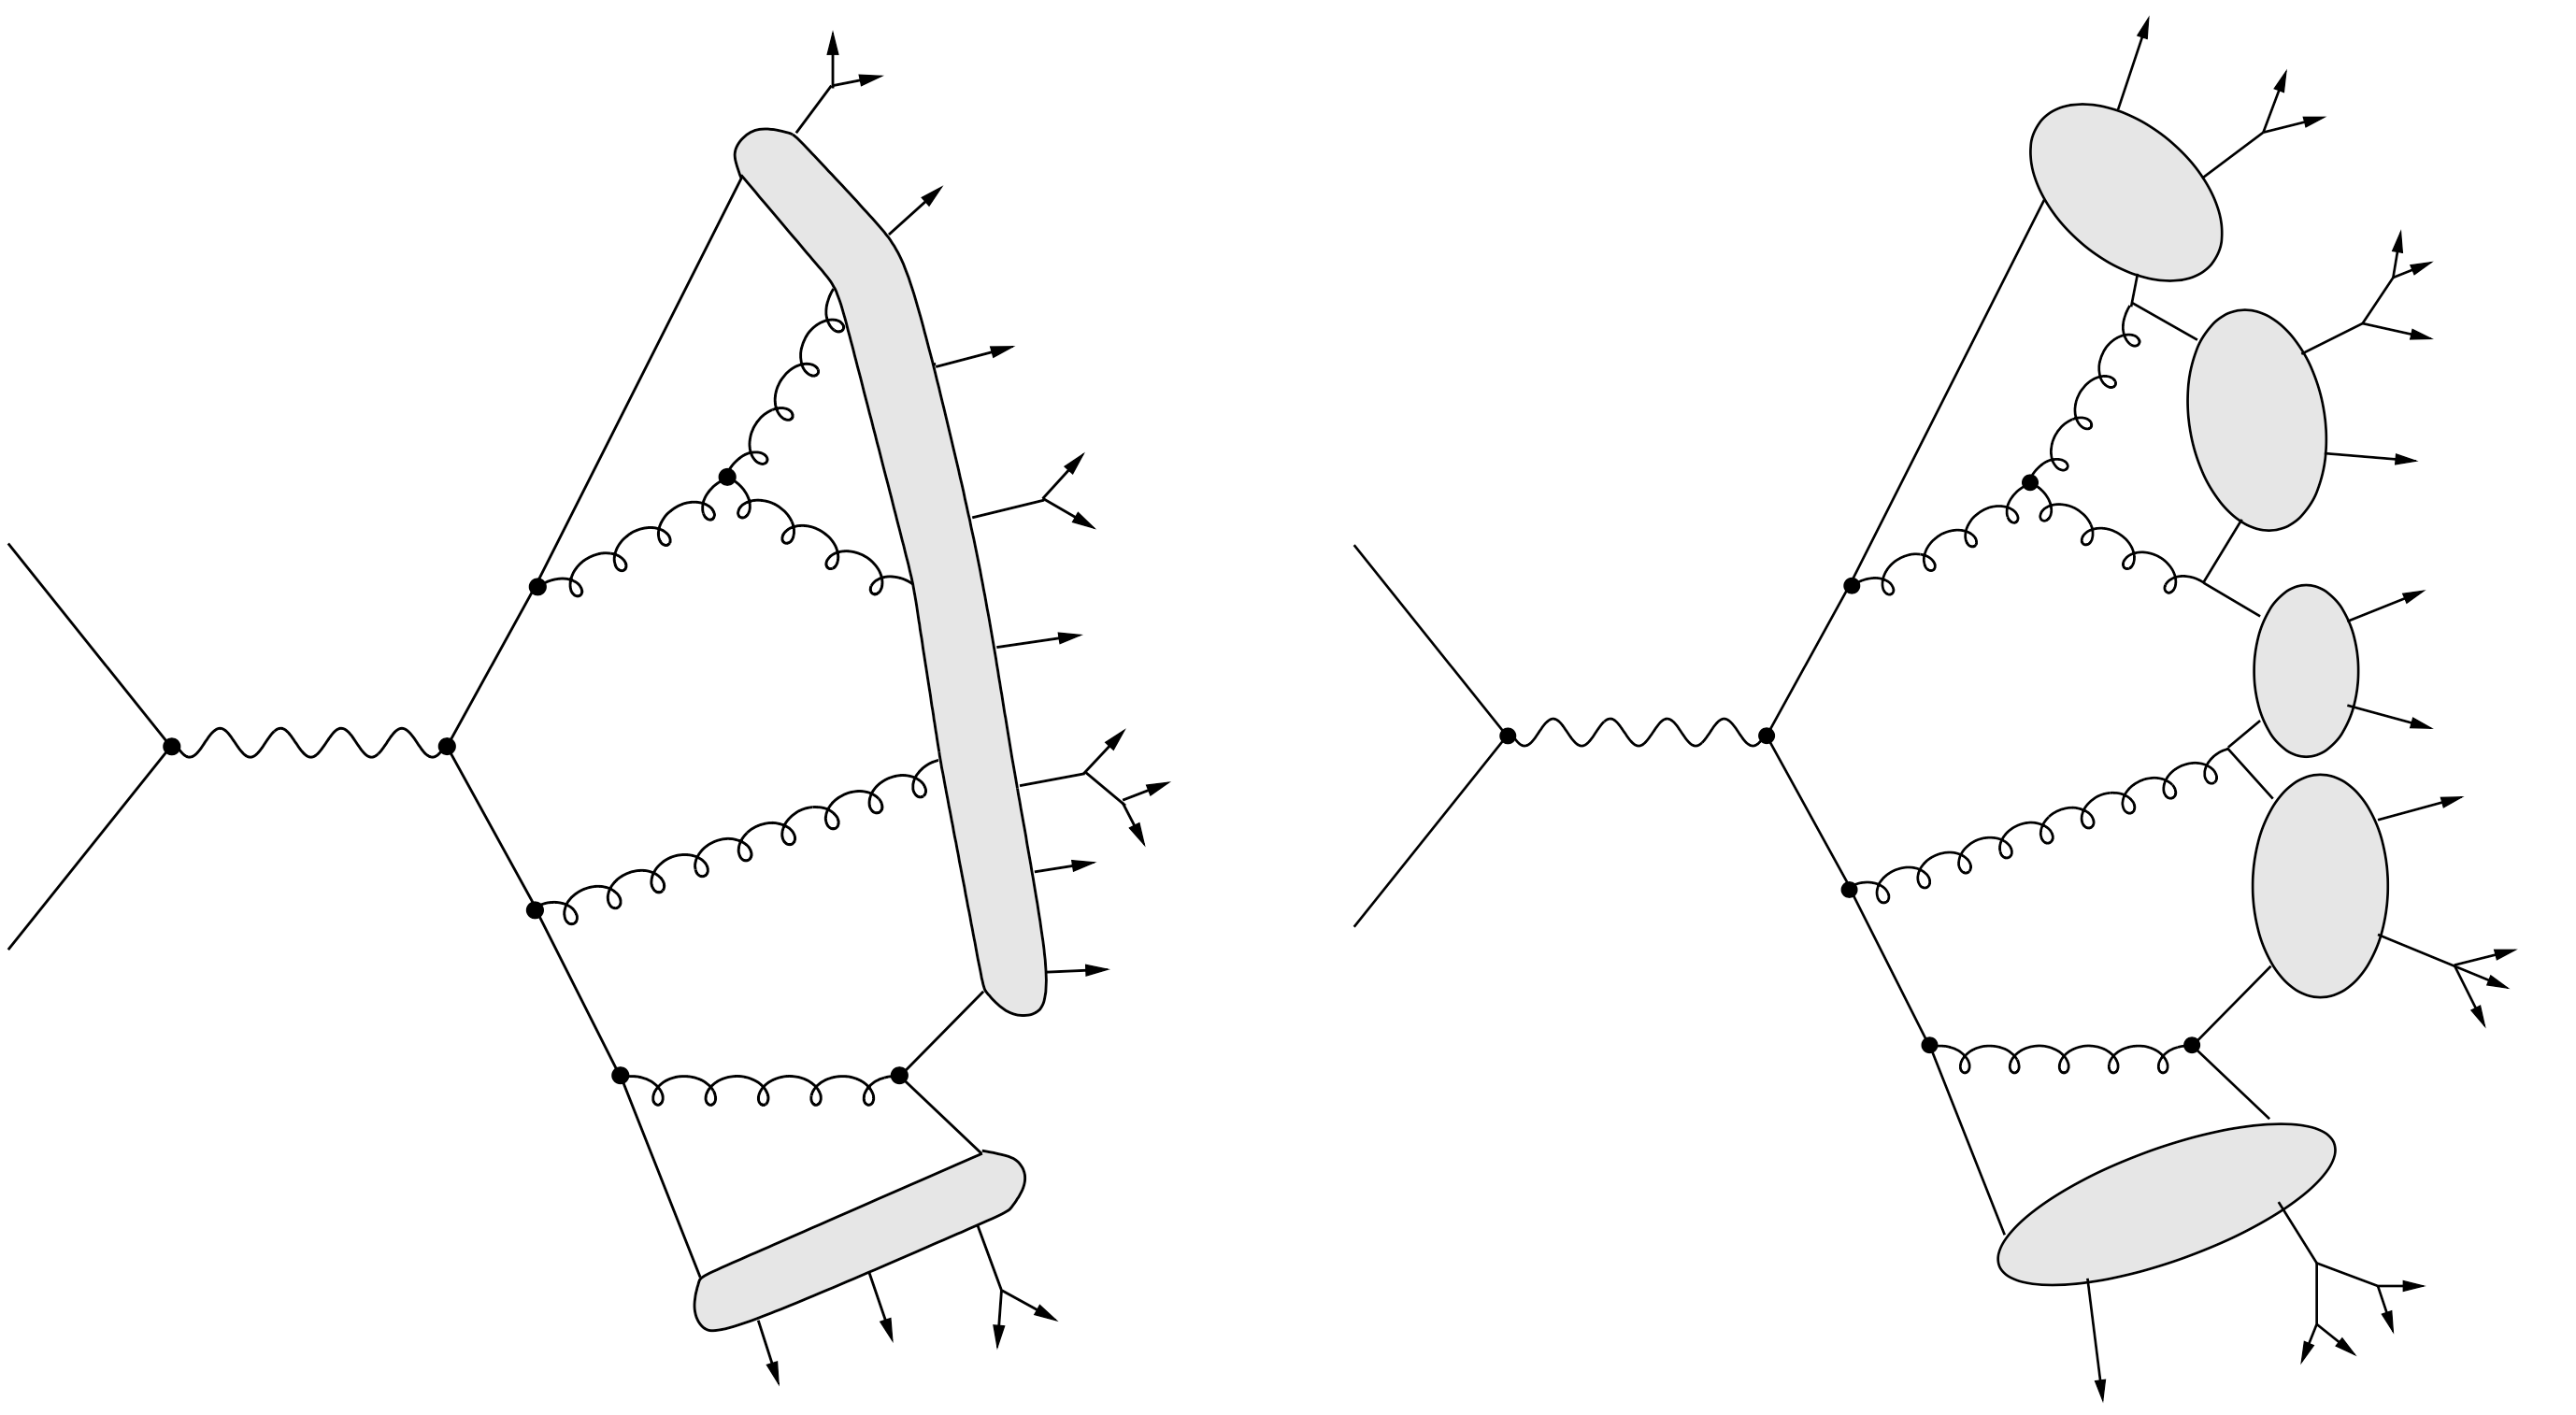
\includegraphics[width=0.5\linewidth]{src/img/hadronization.png}
    \caption[Illustration of the hadronization models. The left is the Lund model, and the right is the cluster fragmentation.]{Illustration of the hadronization models. The left is the Lund model, and the right is the cluster fragmentation. \footnotemark}
    \label{fig:hadronization}
\end{figure}
\footnotetext{\url{https://arxiv.org/abs/1011.5131}}

\section{Jets}
\label{sec:jet}
As seen in \cref{sec:IR_div}, partons emit soft and collinear gluons.
The initial momentum of the parton is split into more partons, creating a shower of partons called \emph{jet}.
The main processes in proton-proton collisions that produce a jet are shown in \cref{fig:qq,fig:qg,fig:gg}.

Experimentally it is not straightforward to define a jet from the measured decays.
For example, a quark initially radiates one collinear gluon, having approximately the same momentum as the quark.
How do you decide whether the gluon is part of the initial jet or creates a new one?
Or, if two jets exchange a soft gluon that emits another one, how do you decide where the new gluon belongs?
This is important because if the jets are not defined correctly, the infinities in the scattering amplitude will not be canceled out, as is stated in the KLN theorem \cite{IR_sing_K,IR_sing_LN}.
This makes analyzing the data very difficult. 

There are complex algorithms that use unique physical variables to enable the reconstruction of the jets \cite{antikt}.
In the first approximation, we can say that the jet is a \emph{cone}, where the apex corresponds to the initial parton and all other partons created are inside the cone. 
We will discuss this in more detail in ????.
The illustration of a jet is shown in \cref{fig:jet}.

Another aspect of jets is the definition of their energy.
The most common approach to defining the jet 4-momentum is by summing the 4-momenta of all the partons inside the jet \cite{antikt}.
The problem is that it introduces a mass to the jet, but the initial parton is massless.

\begin{figure}[htb]
    \centering
    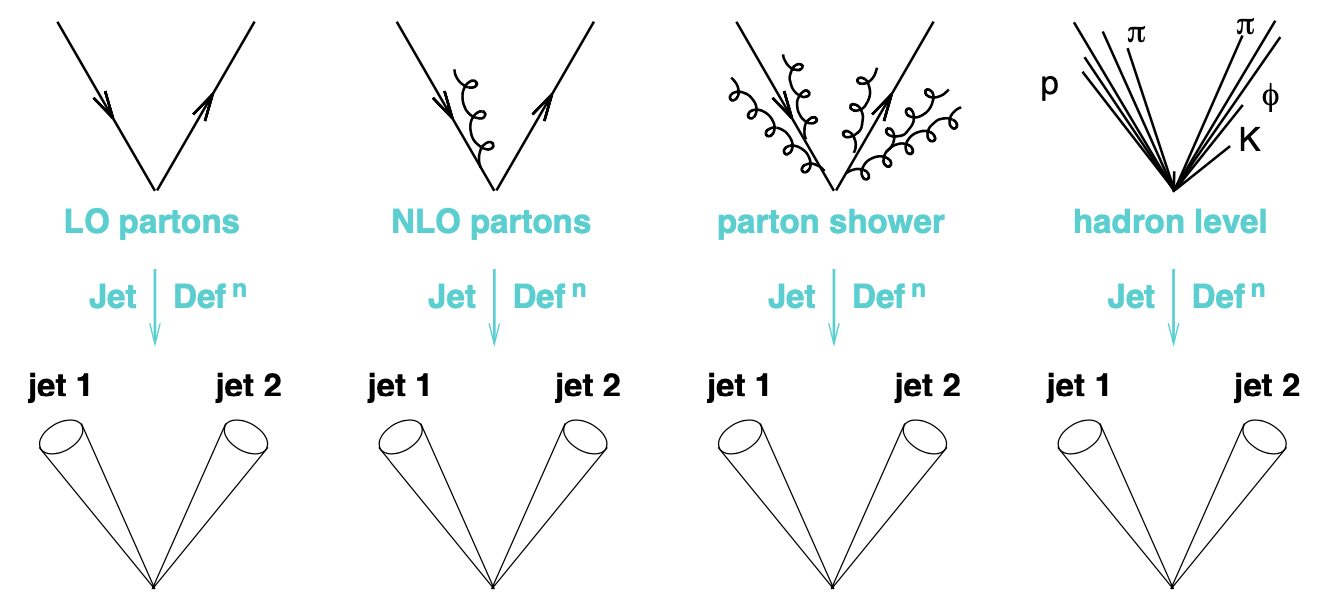
\includegraphics[width=0.7\linewidth]{src/img/jet.png}
    \caption[Jet definitions on various levels.]{Jet definitions on various levels. LO refers to the leading order in perturbation, and NLO to the next-to-leading order.\footnotemark}
    \label{fig:jet}
\end{figure}
\footnotetext{\url{https://arxiv.org/abs/1011.5131}}

\subsection{Infrared and Collinear Safety}
\label{sec:IR_coll_safe}
One way of making sure that the jet algorithm is reflecting the physics of partons is to make sure that the jet algorithm is \emph{infrared and collinear safe}:
\begin{itemize}
    \item \textbf{Collinear safety} means that if the initial parton (or any other in the shower) radiates a \emph{collinear} gluon, it is always part of the same jet.
    \item \textbf{Infrared safety} means that the jet is unchanged if the initial parton (or any other in the shower) radiates a \emph{soft} gluon.
\end{itemize}

In \cref{fig:collinear_safety}, we can see that the jet algorithm initially finds two jets, but when one jet radiates a soft gluon, they are put together.

\begin{figure}[htb]
    \centering
    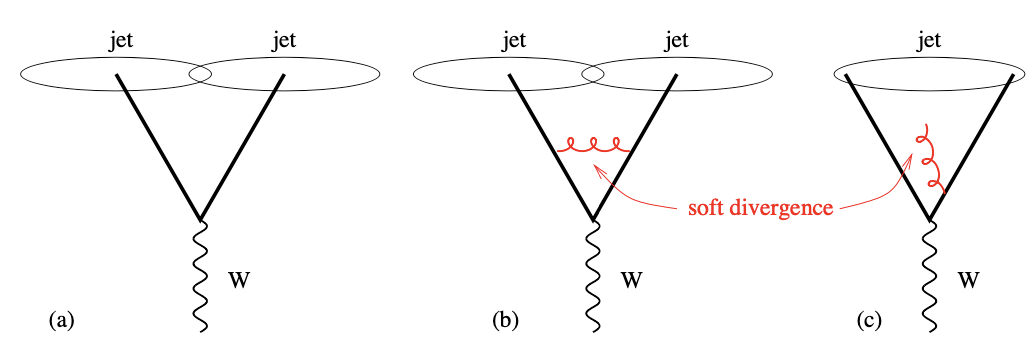
\includegraphics[width=0.7\linewidth]{src/img/collinear_safety.png}
    \caption{Collinear unsafe jet algorithm. Initially, there are two jets, but they are put together if one jet radiates a soft gluon.}
    \label{fig:collinear_safety}
\end{figure}